\begin{figure}[H]
    \centering
    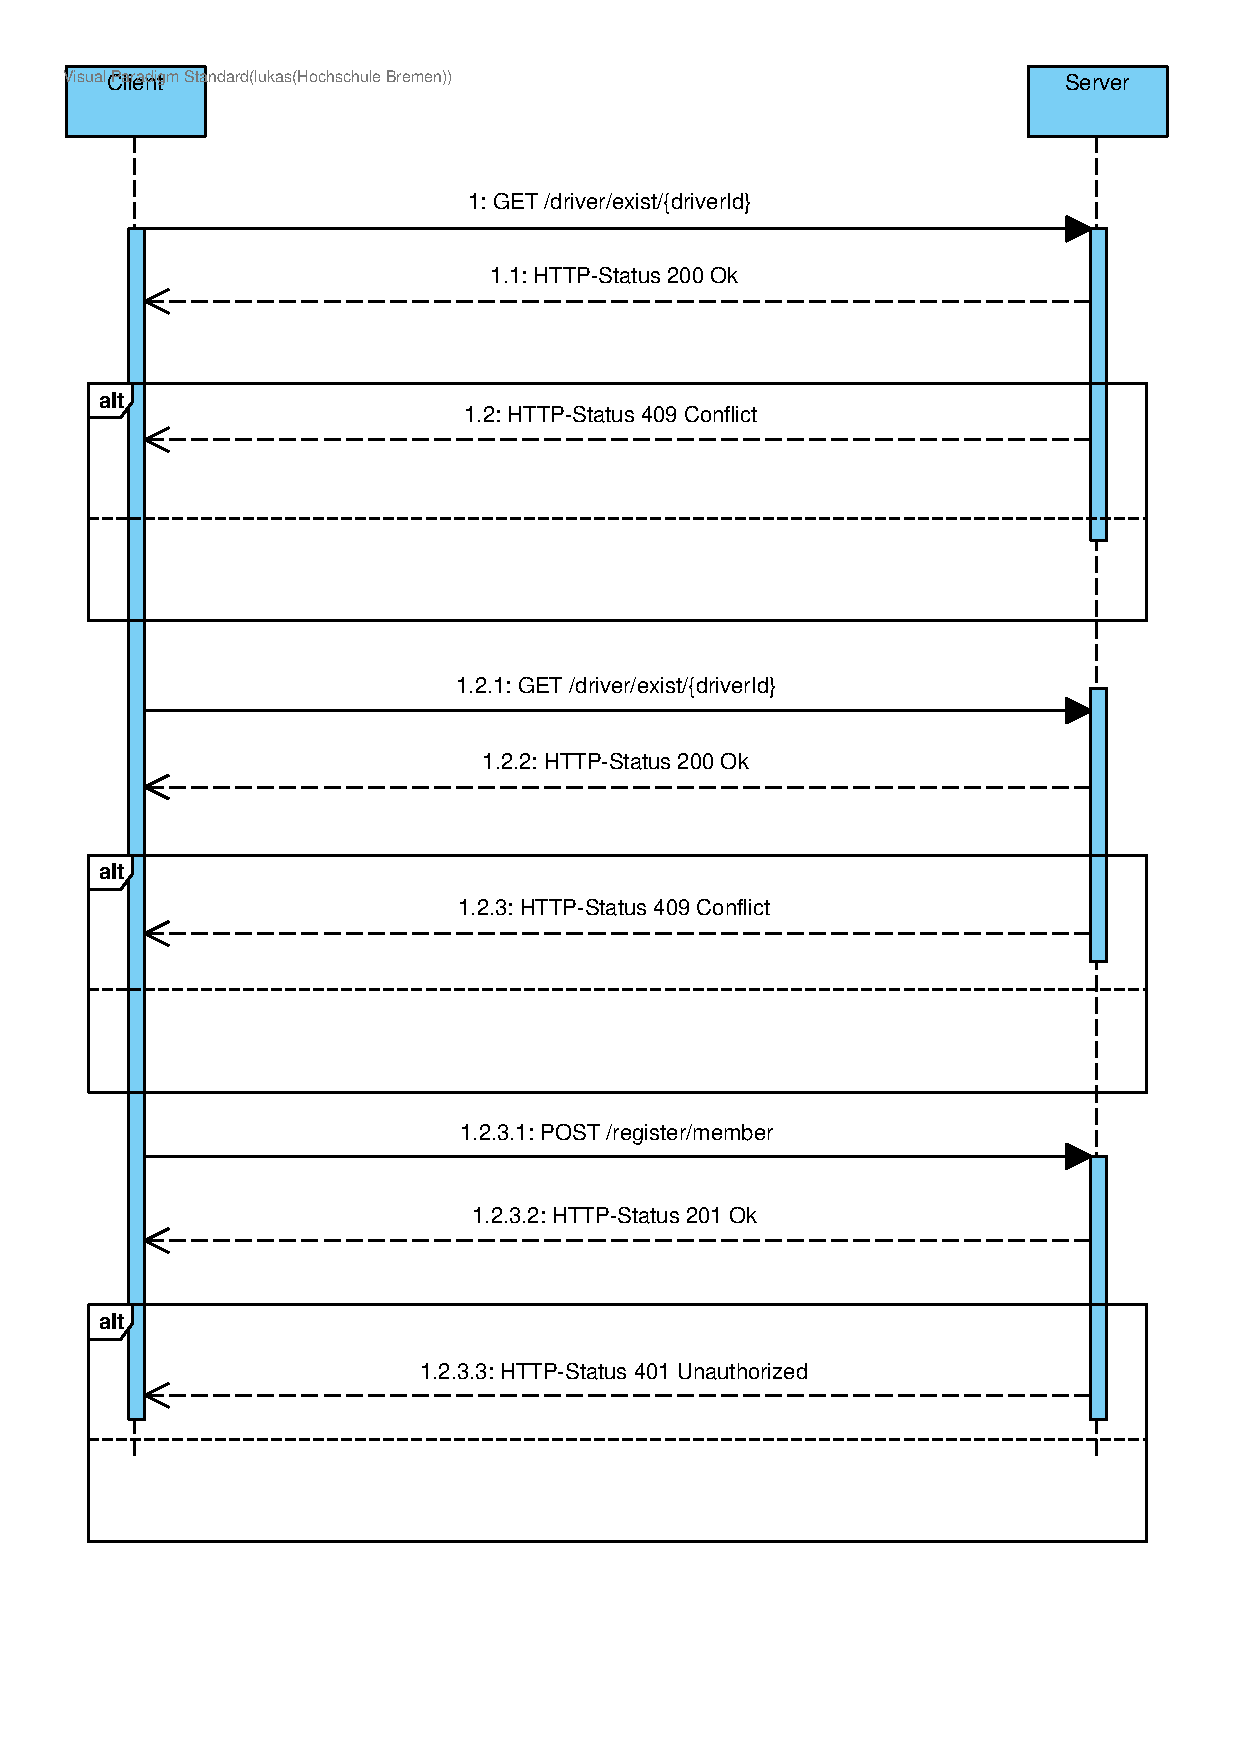
\includegraphics[width = 0.87\textwidth]{pictures/fastlane_sequenz_diagramm}
    \caption{Sequenzdiagramm}
    \label{fig:sequenzdiagramm}
\end{figure}

Das abgebildete Sequenzdiagramm stellt den Vorgang des Registrierens dar.
Dabei ist zu beachten, dass die Requests an die entsprechende Serveradresse gesendet werden.
Somit würde beispielsweise ein vollständiger Request an die localhost Adresse, über den Port 8080 folgendermaßen
aussehen: http://localhost:8080/driver/exist/licenseId.
Zu Beginn der Registrierung muss der Nutzer seine Führerschein Id eingeben.
Daher wird ein HTTP-Request an das Backend an den Endpunkt \enquote{/driver/exist/licenseId} gesendet.
Existiert die Führerschein Id noch nicht, so wird der Status Code 200 Ok zurückgesendet.
Ist die Id allerdings schon im System vorhanden, wir der Status Code 409 Conflict
zurückgesendet. \medskip

Zu einem späteren Zeitpunkt der Registrierung wird vom Benutzer eine E-Mail eingegeben.
Dabei läuft der gleiche Prozess erneut ab.
Es wird ein HTTP-Request an den Endpunkt \enquote{account/exist/email} gesendet.
Wenn die E-Mail bereits im System existiert, wird der Status Code 409 Conflict zurückgesendet.
Existiert sie allerdings noch nicht, wird der Status Code 200 Ok gesendet. \medskip

Sobald der Nutzer mit der Eingabe seiner Daten fertig ist, wird ein Post Request an den
Endpunkt \enquote{/register/member} gesendet.
Dabei werden im Body des Requests alle eingegebenen Daten mitgegeben.
Sofern die Registrierung im Backend erfolgreich verläuft, wird der Status Code 201 Created gesendet.
Tritt jedoch ein Fehler auf, wird der Status Code 401 Unauthorized zurückgesendet. \medskip

Dieses Diagramm stellt nur die Registrierung dar, allerdings laufen die meisten Prozesse nach dem gleichen Prinzip
ab.
Sobald im Frontend ein Request gesendet wird, wird dieser im Backend verarbeitet und der Entsprechende Status Code
mit dem Passenden Body zurückgesendet.